\documentclass[../Bachelorarbeit.tex]{subfiles}

\begin{document}
\section{Event selection}
\label{sec:Event_selection}
\begin{table}[h]
    \begin{tabular}{  l c c c }
        \hline
        Event selection criterion                 & lllvjj region & WZjj region & VBSSR   \\
        \hline
        Event cleaning                            & $\surd$       & $\surd$     & $\surd$ \\
        GoodRunList                               & $\surd$       & $\surd$     & $\surd$ \\
        Trigger                                   & $\surd$       & $\surd$     & $\surd$ \\
        Primary Vertex                            & $\surd$       & $\surd$     & $\surd$ \\
        \hline
        lllvjj finale state                       &               &             &         \\
        \qquad $\geq 2$ jets                      & $\surd$       & $\surd$     & $\surd$ \\
        \qquad $\geq 3$ Z-Analysis leptons        & $\surd$       & $\surd$     & $\surd$ \\
        \qquad One SFOC pair                      & $\surd$       & $\surd$     & $\surd$ \\
        $l_{W}$ is in W-Analysis selection        & $\surd$       & $\surd$     & $\surd$ \\
        Transverse momentum of leading leptons    &               &             &         \\
        \qquad $p_{T}(l)>25(27) GeV$              & $\surd$       & $\surd$     & $\surd$ \\
        Transverse momentum of subleading jet     &               &             &         \\
        \qquad $p_{T}(j_{2})>40 GeV$              & $\surd$       & $\surd$     & $\surd$ \\
        \hline
        $M_{T}(W)>30 GeV$                         &               & $\surd$     & $\surd$ \\
        $\lvert M(ll)-91.1876 GeV\rvert < 10 GeV$ &               & $\surd$     & $\surd$ \\
        four Baseline leptons veto                &               & $\surd$     & $\surd$ \\
        b-jet veto                                &               & $\surd$     & $\surd$ \\
        \hline
        $M(jj)>500 GeV$                           &               &             & $\surd$ \\
        $\Delta Y(jj) >2$                         &               &             & $\surd$ \\
        \hline
    \end{tabular}
    \centering
    \caption{Schematic view of cuts applied in different phase space regions. \cite{Bittrich.27.05.2020}}
    \label{tab:eventselection}
\end{table}

Event Selection is done in order to degrease background and get a clean signal process. VBS processes have
a small cross-section around 1 fb resulting in a small event count. In the 2015 and 2016 Atlas
run with 36 $fb^{-1}$ not even 100 events produce VBS processes.
There for one has to carefully select Events in order to get a meaningful signal process. The Events Selection is implemented
as described in \cite{Bittrich.27.05.2020} using the Common Analysis Framework(CAF). The Object selection however was already done in ELCore
and account for the Event cleaning, GoodRunList, Trigger, Primary Vertex in Table \ref{tab:eventselection} these cant be change in the CAF.
Therefore, only the Event selection done in the CAF will be discussed. ELCore produces beam reconstruction
level samples the Event Selection in the CAF is split into the three phase space regions lllvjj, WZjj and the VBS signal region(VBSSR).
Even though the regions are different the selection criteria overlap. The WZjj region use the selection criteria of
the lllvjj as base and introduces new selection criteria.
The same is true for the VBSSR which builds upon the WZjj region as show in Table \ref{tab:eventselection}.
\\\\
\textbf{lllvjj region:} Only events with 3 or more leptons that pass the Z-analysis are chosen. The Leptons are then assigned to the decaying gauge boson.
For this same flavour and opposite charge(SFOC) leptons pairs are chosen. The pair with invariant mass close to the Z Boson mass is assigned to the Z-Boson.
The highest transverse momentum $p_{T}$ lepton from the remaining leptons is assigned to the $W^{\pm}$-Boson and required to pass de W-analysis.
Chosen leptons need a transverse momentum $p_{T} > 25(27)$ GeV for the 2015(2016) campaign for the events to pass the trigger threshold.
Events have to have two or more events in order to be selected. These jets need to have $p_{T}(j)>40$ GeV to be considered as tagging jets.
\\\\
\textbf{WZjj region:} Additinal cuts are applied for the WZjj region in order to maximise $W^{\pm}Z$ contribution in the lllvjj final state.
Some Events line ZZ diboson production are expected to produce an additional lepton therefore a four lepton Baseline veto is applied.
Events where the jet is considered a b-jet are discarded to minimize $t\bar{t}$ and other t-quark contributions.
The Transverse mass of the $W{\pm}$-Boson is required to be greater than $M_{T}(W)>30$ GeV.
The Z lepton pair has to have an invariant mass within 10 GeV of the Z-Boson mass $m_{Z}=91.1876$.
\\\\
\textbf{VBSSR region:} The resonance fitting is done in the VBSSR region. For this additional requirements must be added
increasing WZjj-EW6 contribution compared to WZjj-EW4 and WZjj-EW5. For this two cuts for the tagging jets have to added. The invariant mass must be
$M(jj)>500$ GeV and the absolute rapidity difference hast be constraint $\Delta Y(jj) >2$.
\\\\

\begin{figure}[h]
    \centering
    \begin{subfigure}{0.45\textwidth}
        \centering
        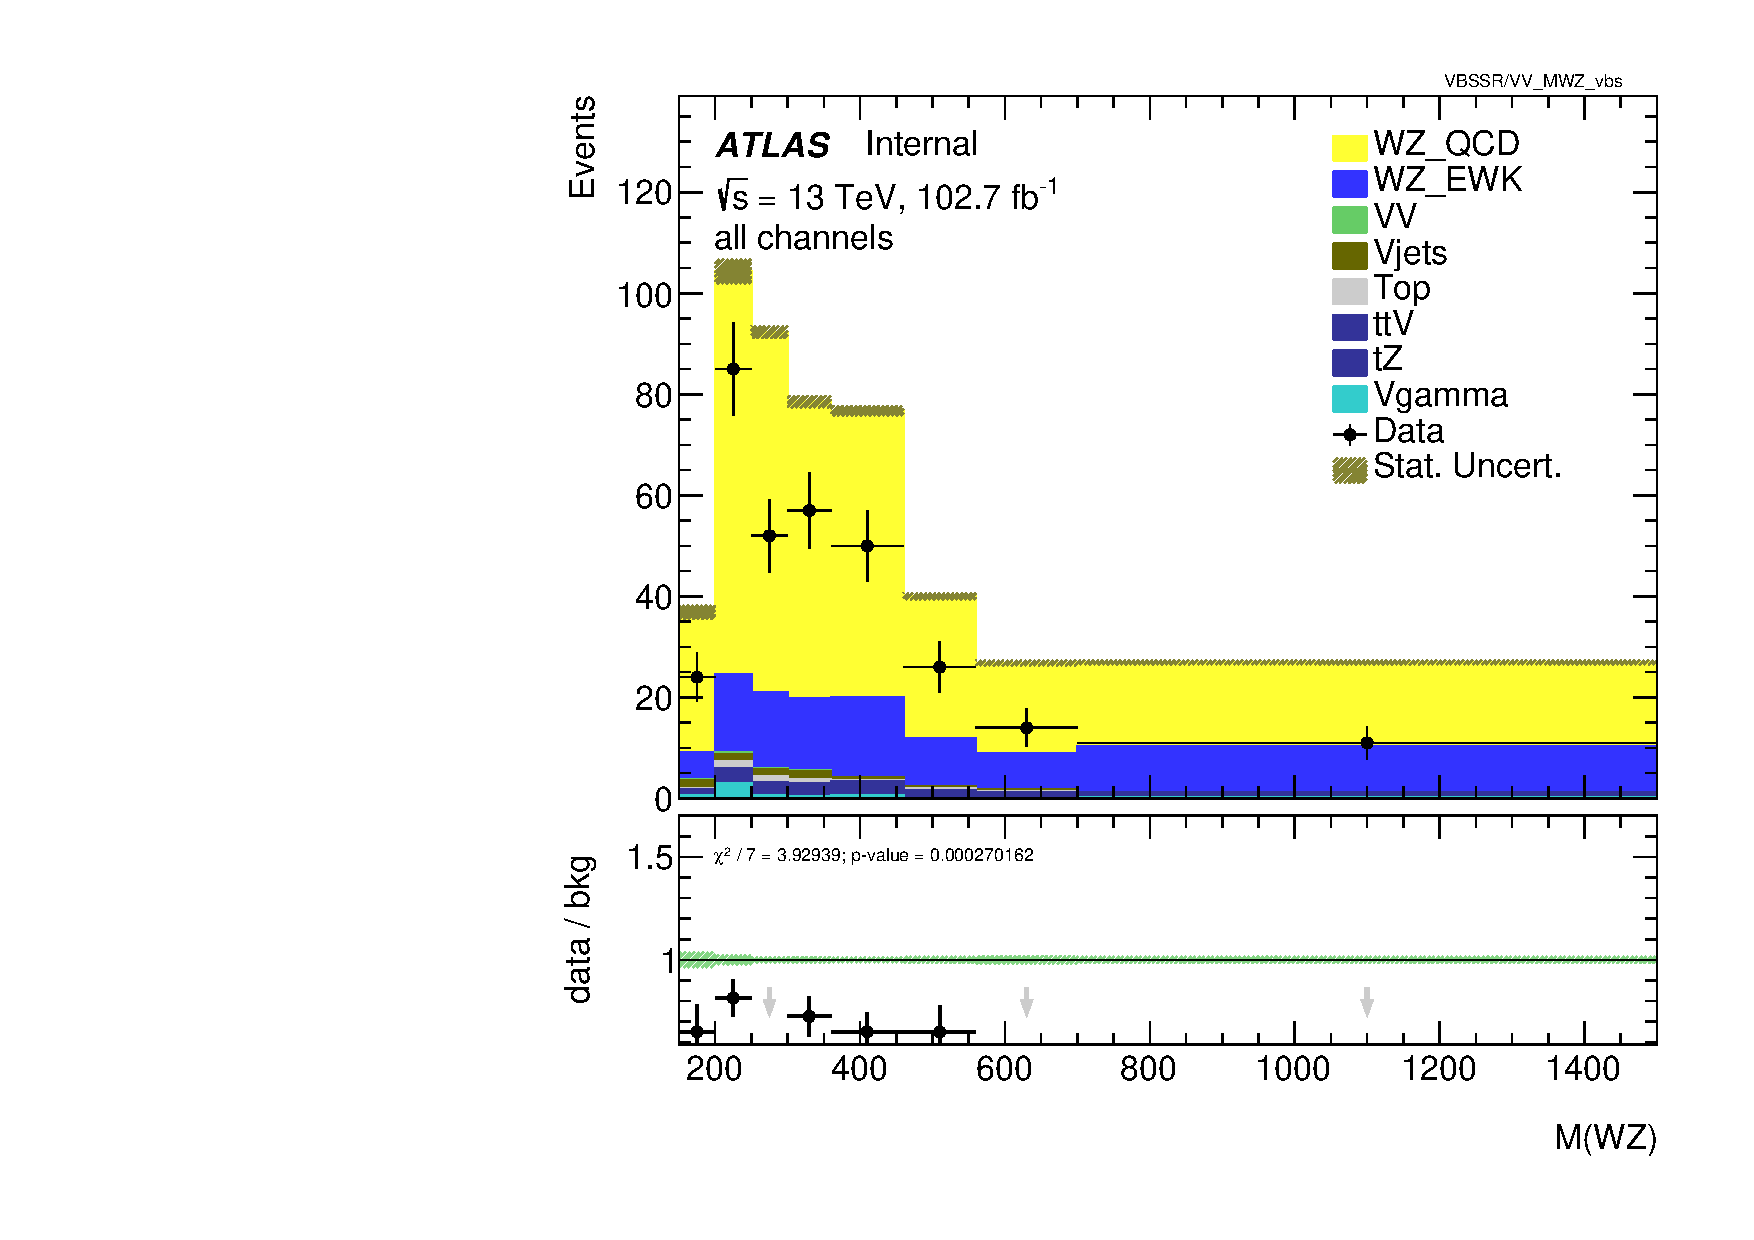
\includegraphics[width=\textwidth]{Plots/SM_reproduction/all_VV_MWZ_vbs.pdf}
        \caption{}
    \end{subfigure}
    \begin{subfigure}{0.45\textwidth}
        \centering
        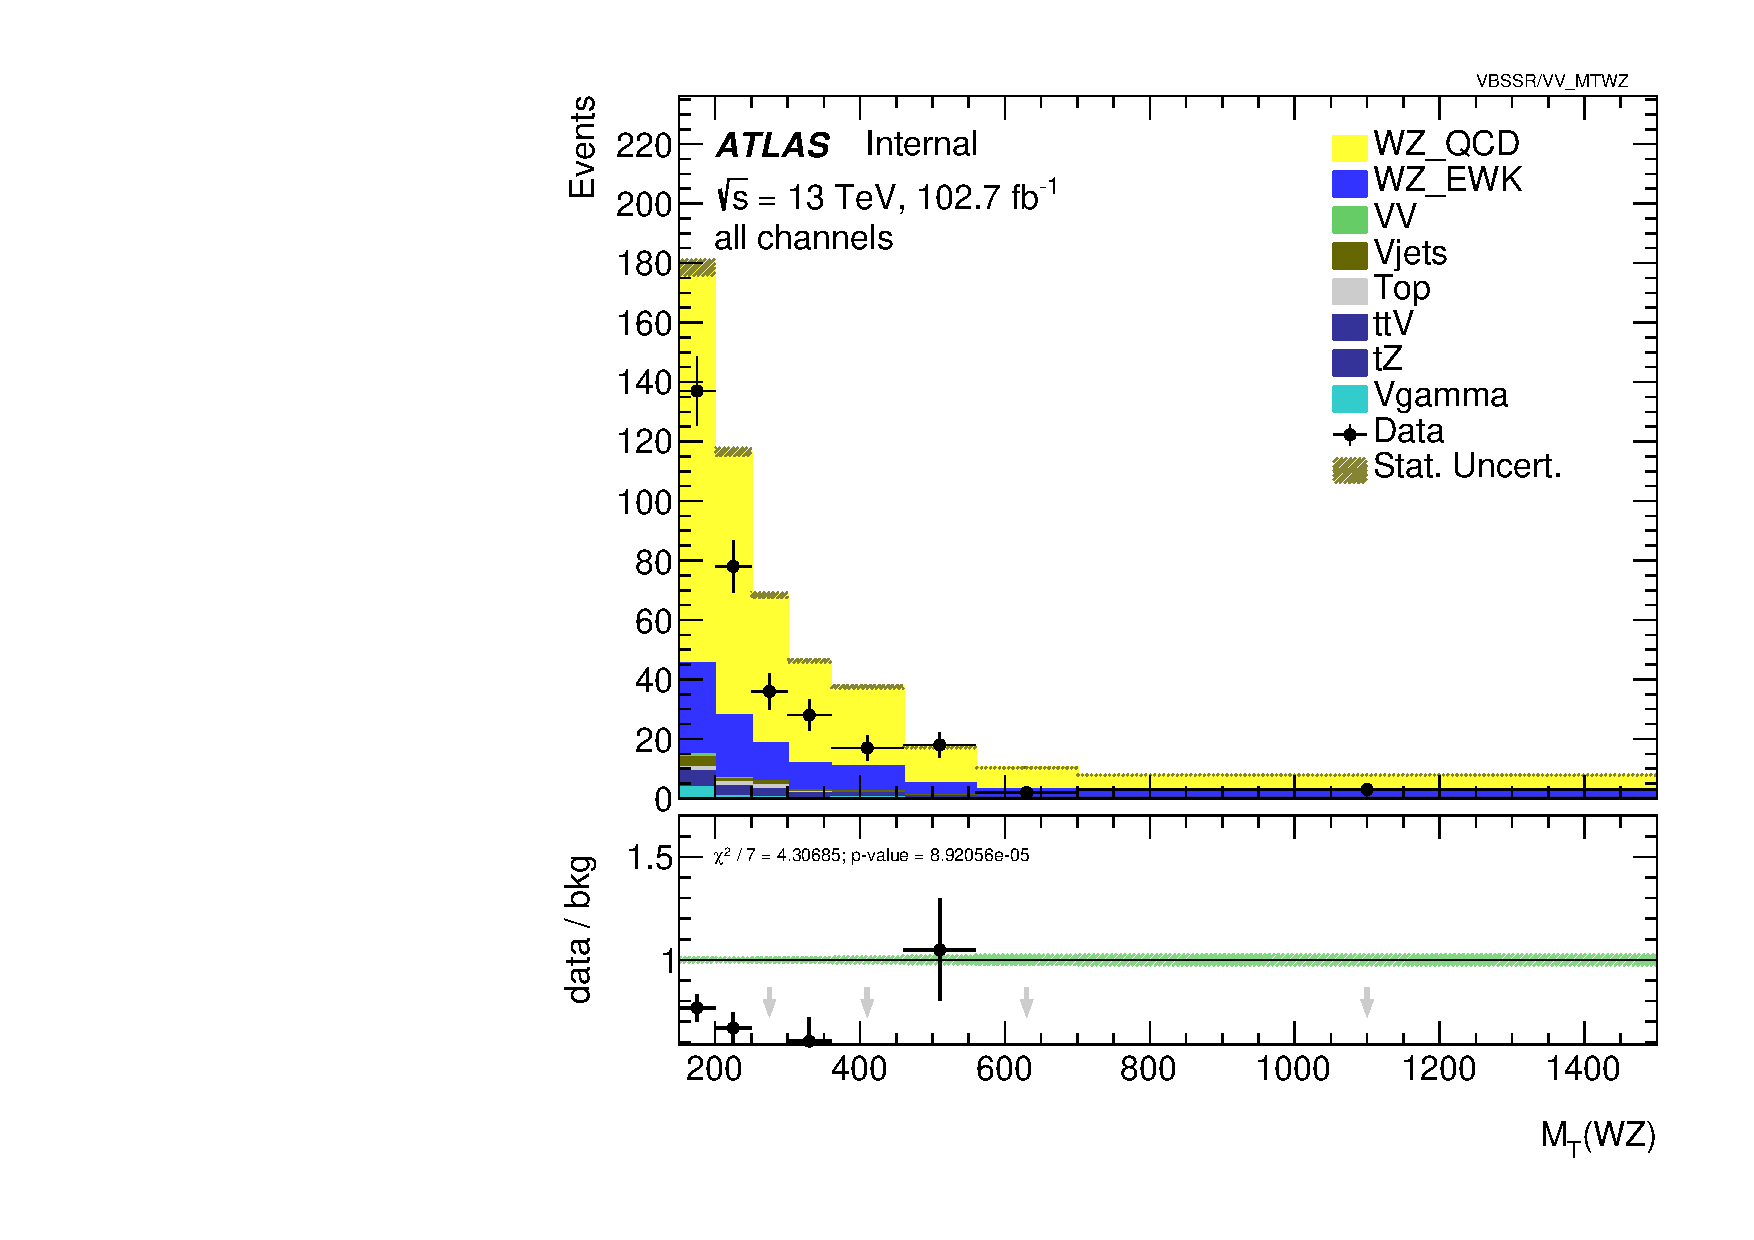
\includegraphics[width=\textwidth]{Plots/SM_reproduction/all_VV_MTWZ.pdf}
        \caption{}
    \end{subfigure}
    \caption{VBSSR region for a) invariant Mass, b) transverse mass. Showing reproduction of SM as well as the in section \ref{sec:VBS} discussed dominance of QCD and EW processes. VV, Vjets, Top, ttV, Vgamma, $WZ\_EWK$, $WZ\_QCD$ are combined to $'WZ\_SM + Background'$ in later plots. For the fits $WZ\_EWK$ is used as signal.}
    \label{fig:SM_re}
\end{figure}

Figure \ref*{fig:SM_re} shows the cuts for the VBSSR region applied for the combined data from mc16d and mc16e with a combined luminosity of 102.7 $fb^{-1}$.
These histograms will be combined to WZ + Background in the following Plots.
Ideally one would use all campaigns mc16a, mc16d and mc16e with combined luminosity of 139 $fb^{-1}$ to achieve the best statistic.
For this Analysis the EFT Samples as well as the GM resonance samples have to be included resulting in to many Branches in the TQSampleTree than
the current ROOT version 6.14.04 used by the CAF can process.


\begin{table}
    \centering
    \begin{tabular}{ l c c c }
        \hline
        VBSSR              & mc16d+mc16e           & mc16a                 & SM             \\
        \hline
        WZ QCD             & $356.8912 \pm 2.4118$ & $121.5475 \pm 1.1721$ & $144 \pm 41$   \\
        WZ EWK             & $91.2393 \pm 0.4231$  & $32.4363 \pm 0.2522$  & $24.9 \pm 1.4$ \\
        Background         & $27.2161 \pm 2.0335$  & $11.9691 \pm 0.4701$  & $31.1 \pm 3.9$ \\
        \hline
        WZ SM + Background & $475.3466 \pm 3.2912$ & $165.9529 \pm 1.4050$ & $200 \pm 41$   \\
        \hline
    \end{tabular}
    \caption{Overwiev of Events in VBSSR region. mc16a is compared to the \cite{Sampsonidou.25.11.2021} for the reproduction of the SM EFT Limits.
        While the Resonance Fitting is done with the mc16e+mc16d data. The differences between the mc16a and the SM is like cause by some ELCore settings
        since the cuts possible in the CAF tool where replicated.}
    \label{tab:SM_re}
\end{table}

\begin{table}
    \centering
    \begin{tabular}{l | c c | c }
        \hline
                 & \multicolumn{2}{c|}{EFT Optimized binning} & SM Optimized Binnnig                  \\
        Operator & $M(WZ)$                                    & $M_{T}(WZ)$          & $M_{T}(WZ)$    \\
        \hline
        S0       & [-49 , 47.4]                               & [-46 , 44.1]         & [-78 , 78]     \\
        M0       & [-9.1 , 11.5]                              & [-9.3 , 9.65]        & [-15 , 15]     \\
        M1       & [-16 , 15.7]                               & [-15 , 14.4]         & [-23 , 23]     \\
        T0       & [-0.43 , 0.457]                            & [-0.38 , 0.325]      & [-1.4 , 1.4]   \\
        T1       & [-0.82 , 0.713]                            & [-0.72 , 0.682]      & [-0.97 , 0.97] \\
        T2       & [-2.4 , 2.16]                              & [-2.2 , 1.96]        & [-2.8 , 2.8]   \\
        \hline
    \end{tabular}
    \caption{Asmiove fit Limits for SM data with $95\%$ CL. Differences arise from the use of mc16e, mc16d data compared to the mc16a data and the use of an BSM search optimized binning compared to the SM optimized binning used in \cite{Sampsonidou.25.11.2021}}
    \label{tab:asimov}
\end{table}

\section{Maxmimum Likelihood Methode}
The fitting tool provides the log-Likelihood function for a given parameter. This is done using the maximum likelihood method. \cite{Prof.Dr.KlausReygersDr.RainerStamen.2020}, \cite{Prof.MarkusSchumacherDr.StanLai.2012} and \cite{K.F.RILEY.} provide an in depth view into the topic, but a short introduction is given here to understand the fitting results.
The maximum likelihood method takes observed data and an assumed probability distribution in order to give the best estimate for a parameter.

The Likelihood function for a joint probability distribution(pdf) is defined as:
\begin{equation}
    L(\overrightarrow{x},\overrightarrow{\Theta}) = \prod_{i=1}^{n} f(x_{i},\overrightarrow{\Theta})
\end{equation}

With distribution $f(x;\overrightarrow{\Theta})$, $\overrightarrow{\Theta} = (\Theta_{1},\Theta_{2},\dots,\Theta_{m})$ and a measurement of n independent values $\overrightarrow{x}=(x_{1},x_{2},\dots,x_{n})$.
The Maxmimum of the Likelihood function is the best estimate for the parameter $\overrightarrow{\Theta}$.
It is often particle to maximize the log-Likelihood function $ln L$. The derivative can be written as follows since the logarithm is a monotonically increasing function.
\begin{equation}
    \frac{\partial L}{\partial \Theta_{i}} \bigg \vert_{\overrightarrow{\Theta}=\hat{\Theta}} = 0 \qquad \Longrightarrow \qquad \frac{\partial ln L}{\partial \Theta_{i}} \bigg \vert_{\overrightarrow{\Theta}=\hat{\Theta}}=0
\end{equation}
Where $\hat{\Theta}$ is the ML estimate. This can be applied to a Gaussian distribution with $E[x_{i}]=\mu(y_{i},\overrightarrow{\Theta})$ and $V[x_{i}]=\sigma_{i}^{2}$

\begin{equation}
    f(x,\overrightarrow{\Theta}) = \frac{1}{\sqrt{2\pi \sigma^{2}}} e^{-\frac{(x-\mu(y_{i},\overrightarrow{\Theta}))^{2}}{2 \sigma^{2}}}
\end{equation}

resulting in a log-Likelihood function

\begin{equation}
    ln \: L(\overrightarrow{\Theta}) = \sum^{n}_{i=1} \left( ln \frac{1}{\sqrt{2\pi}}-ln \: \sigma - \frac{(x_{i} - \mu(y_{i},\overrightarrow{\Theta}))^2}{2 \sigma^{2}}\right)
\end{equation}
Only $\mu$ is dependent in the parameter on $\overrightarrow{\Theta}$ and therefore only the third therm is relevant. One can now compare the result to the chi-squared method
\begin{equation}
    \chi^{2}(\overrightarrow{\Theta}) = \sum^{n}_{i=1} \frac{(x_{i} - \mu(y_{i},\overrightarrow{\Theta}))^2}{\sigma^{2}}
\end{equation}
And the log-Likelihood function can therefore be written as $-2 ln \: L = \chi^{2}$. If $x_{i}$ isn't Gaussian distributed than the chi-squared method is an "ad hoc" method.
This form has the advantage that if a gaussian distribution is assumed the parameters can be easily determined but can give asymmetric uncertainties.
The standard deviation can be calculated by setting the derivative of L with respective to $\sigma$ and derivative of L with respective to $\mu$ equal to zero.

\begin{equation}
    \frac{\partial ln L}{\partial \mu} = \sum_{i = 1}^{N} \frac{x_{i}-\mu}{\sigma^{2}} = 0
\end{equation}

\begin{equation}
    \frac{\partial ln L}{\partial \sigma} = \sum_{i = 1}^{N} \frac{(x_{i}-\mu)^{2}}{\sigma_{i}^{3}} - \frac{1}{\sigma} = 0
\end{equation}
These to equations can now be solved simultaneously leading to
\begin{equation}
    \mu = \frac{1}{N} \sum^{N}_{i = 1} x_{i} = \overline{x} \qquad \textnormal{ and } \qquad \sigma^{2} = \frac{1}{N} \sum^{N}_{i = 1} (x_{i}-\overline{x})^{2} = n
\end{equation}
With this the one sigma and two sigma environment can be calculated for a negative log-likelihood function as $1\sigma=1$ and $2\sigma=4$ \cite{Maritn erdman}
\subsection{Likelihood ratio test}
The likelihood-ratio test is used to estimate the goodness of fit based on their likelihoods. In general the denominator contains the likelihood for the entire parameter space, while numerator introduces constrains on the parameter space.
\begin{equation}
    \lambda(\epsilon) = \frac{L(\epsilon,\overrightarrow{\Theta}_{0})}{L(\epsilon,\hat{\Theta})}
\end{equation}
where $\overrightarrow{\Theta}_{0}$ donates the value $\overrightarrow{\Theta}$ for which L is maximized for a given $\epsilon$. $\epsilon$ is the
conditional maximum-likelihood estimator of $\Theta$. In case of the log-likelihood function this can be written as:

\begin{equation}
    \lambda = -2(ln(\frac{L(A)}{L(B)})= -2(ln L(A)-ln L(B))=-2 \Delta L
\end{equation}
In the context of fitting in EFT $L(A)$ donates a fixed parameter while $L(B)$ donates the floating parameter. The likelihood-ratio is than plotted against the parameter values  \ref{fig:S1_with_fit_diffrence_225}.
\end{document}
